% load relevant packages
\documentclass[11pt,a4paper]{article}
\usepackage[hyperref]{acl2020}
\usepackage{times}
\usepackage{amsmath}
\usepackage{amssymb}
\usepackage{mathtools}
\usepackage{latexsym}
\usepackage{lipsum}
\usepackage{graphicx}
\graphicspath{{../../img/}}
\renewcommand{\UrlFont}{\ttfamily\small}
\usepackage{microtype}
\aclfinalcopy
%\setlength\titlebox{5cm}
\newcommand\BibTeX{B\textsc{ib}\TeX}

% administrative details
\title{Investigating the isometric properties of Neural Machine Translation models on binary semantic-equivalence spaces}
\author{Atreya Shankar \\
  Cognitive Systems, University of Potsdam \\
  Department of Computational Linguistics, University of Zürich \\
  \texttt{atreya.shankar@\{uni-potsdam.de,uzh.ch\}}}
\date{\today}

% start document
\begin{document}

% produce title
\maketitle

% abstract
\begin{abstract}
  \textit{Isometry} is defined mathematically as a distance-preserving transformation between two metric spaces. In this research, we hypothesize that well-performing Neural Machine Translation (NMT) models function approximately isometrically on semantic metric spaces. That is to say, if two sentences are semantically equivalent on the source side, they should remain semantically equivalent after translation on the target side. We begin by utilizing two NMT models of varying performance to translate semantically-equivalent paraphrases based off WMT19 test data references. In order to quantify and simplify the notion of a semantic metric space, we treat it as a probabilistic binary semantic-equivalence space indicating either semantic equality or inequality; achieved by fine-tuning three transformer-based language models on Google's PAWS-X paraphrase detection task. By using the paraphrase detection outputs, we investigate the frequency and composition of semantically isometric behaviour in the NMT models' inputs and outputs.
\end{abstract}

% body
\section{Introduction}

\textit{Isometry} is defined mathematically as a distance-preserving transformation between two metric spaces \cite{coxeter1961introduction}. In this research, we view Neural Machine Translation (NMT) models from the perspective of semantic isometry and hypothesize that well-performing NMT models function approximately isometrically on semantic metric spaces. That is to say, if two sentences are semantically equivalent on the source side, they should remain semantically equivalent after translation on the target side given a well-performing NMT model. A simplified illustration of isometry in higher dimensional functional spaces can be seen in Figure \ref{isometry_visual}.

In order to conduct our investigation, we start by acquiring semantically equivalent paraphrases of WMT19 legacy and additional test references from \citet{freitag-bleu-paraphrase-references-2020} for \texttt{en$\xleftrightarrow{}$de}. Next, we utilize two NMT models of varying performance, specifically FAIR's WMT19 winning single transformer \cite{ng2019facebook} and the Scaling NMT WMT16 Transformer \cite{ott2018scaling}, in order to translate the aforementioned paraphrases in the \texttt{de$\rightarrow$en} translation direction. We use the former model pre-trained from \texttt{fairseq} and train the latter model from scratch.

\begin{figure}
  \centering
  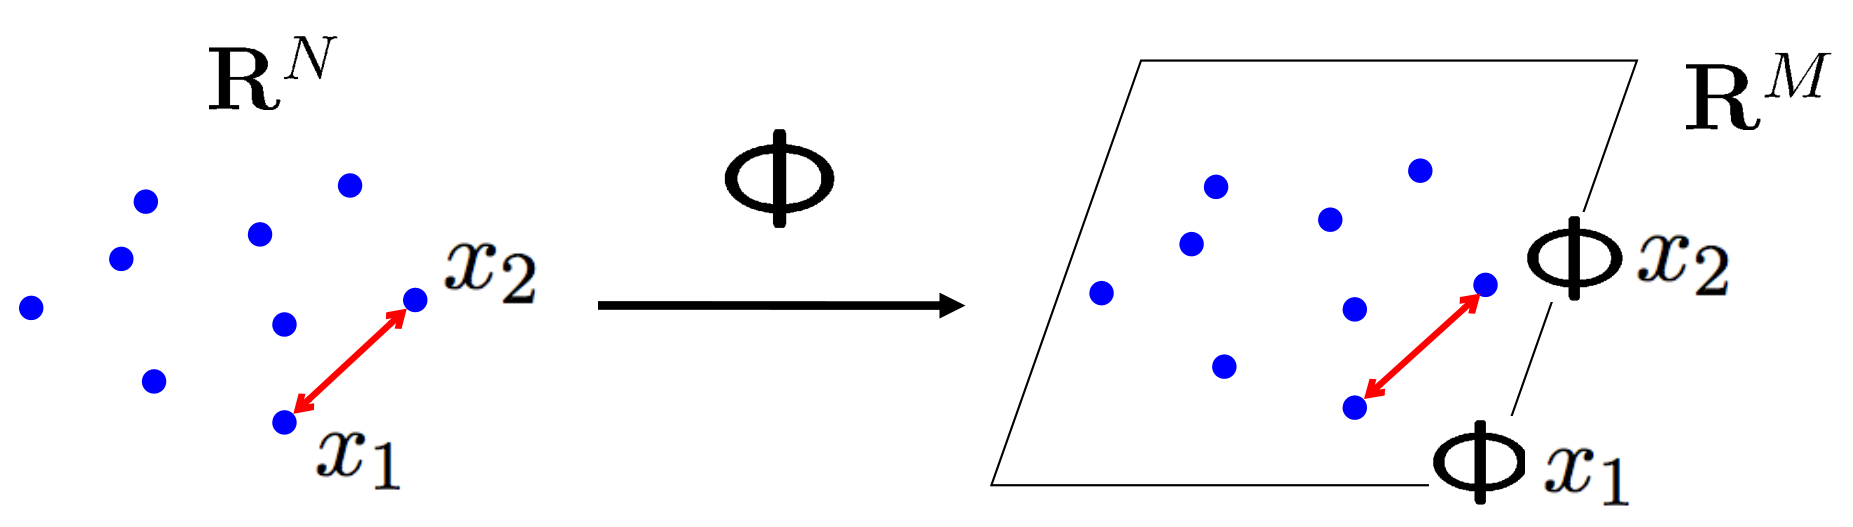
\includegraphics[trim={1.0cm 0cm 0cm 1.0cm},clip,width=0.52\textwidth]{isometry_visualized.png}
  \caption{Illustration of isometry in higher dimensional functional transformations \citep{Hegde-Numax}}
  \label{isometry_visual}
\end{figure}

Next, we utilize three well-performing paraphrase detection models to approximate isometry in the NMT models' translations. These paraphrase detection models are based off mBERT\textsubscript{Base} \cite{devlin2018bert}, XLM-R\textsubscript{Base} and XLM-R\textsubscript{Large} \cite{conneau2019unsupervised} pre-trained multilingual language models; which are correspondingly fine-tuned on Google's PAWS-X paraphrase detection task \cite{pawsx2019emnlp, hu2020xtreme}.
 
Using the outputs of the paraphrase detection models, we finally investigate the frequency and composition of semantically isometric behaviour in the NMT models' inputs and outputs.

% 1. Introduction
% TODO most importantly, add contributions post-paper as concretely as possible -> also add into abstract -> can be done at the end after everything is made clear
% TODO perhaps state expectations more concretely here and in abstract
% TODO perhaps state hypothesis more clearly that isometry is positively correlated with general performance of a model -> perhaps show this statistically where possible with appropriate statistical test
% TODO think of title and how this links up with everything -> change it to reflect content of paper if necessary
% make abstract more similar to introduction where possible

\section{Isometry and approximations}

The concept of isometry in the context of semantic metric spaces can be \textit{exactly} expressed as follows; where $s_i \in \mathbb{R}^{V \times N}$ refers to an input sentence's tokenized matrix-form for vocabulary size $V$ and sentence length $N$, $f: \mathbb{R}^{V \times N} \to \mathbb{R}^{V' \times N'}$ refers to the NMT model's inference function and $D_L: \mathbb{R}^{V \times 2N} \to \mathbb{R}_+$ refers to a semantic distance metric function for language $L$ corresponding to the language of the respective sentences:

\begin{equation}  
  \label{exact_isometry_eqn}
  D_Y(f(s_1),f(s_2)) = D_X(s_1,s_2)
\end{equation}

While elegant, this representation of isometry and a semantic distance metric is problematic. Firstly, exact isometry might not be a practical condition to achieve given real-life data instances with stochastic noise. Next, constructing continuous semantic metric spaces from discrete textual data is a difficult task and is in itself a developing field of research \cite{cer2017semeval}.

\paragraph{Approximate isometry:} To address the first issue, we loosen the constraints of exact isometry to \textit{approximate} isometry:

\begin{equation} 
  \label{approx_isometry_eqn}
  D_Y(f(s_1),f(s_2)) \approx D_X(s_1,s_2) 
\end{equation}

With this approximation, we can simplify the isometric relationship further into a binary semantic-equivalence function $S_L: \mathbb{R}^{V \times 2N} \to \{0,1\}$, which compresses semantic distance metrics to semantic equality ($S_L=1$) or inequality ($S_L=0$) depending on some variable threshold $\delta_L \in \mathbb{R}_+$:

\begin{equation}
  \label{bounded_isometry_eqn}
  S_L(s_1,s_2) =
  \begin{cases}
    1, &D_L(s_1,s_2) \leq \delta_L \\
    0, &D_L(s_1,s_2) > \delta_L
  \end{cases}
\end{equation}

It is worth noting that the formulation in $S_L$ is more meaningful for inferring isometry from semantic equality than from semantic inequality, due to the presence of a tighter bound for the former than the latter.

\paragraph{Probabilistic semantic-equivalence spaces:} To address the second issue, we effectively delegate away the actual computation of a semantic distance metric and convert this into a probabilistic process; with a new definition for $S_L$ below given a probability threshold $\epsilon$. This reformulation allows for the utility of statistical paraphrase detection models without explicit computation of semantic metric spaces. 

\begin{equation}
  \label{bounded_isometry_probability_eqn}
  S_L(s_1,s_2) =
  \begin{cases}
    1, &P\big(D_L(s_1,s_2) \leq \delta_L\big) \geq \epsilon \\
    0, &P\big(D_L(s_1,s_2) \leq \delta_L\big) < \epsilon
  \end{cases}
\end{equation}

With the aforementioned simplifications, we now re-write our equation for approximate isometry as follows:

\begin{equation}  
  \label{exact_approx_isometry_eqn}
  S_Y(f(s_1),f(s_2)) = S_X(s_1,s_2)
\end{equation}

% 2. Motivation (or more thematic title)
% TODO extrapolate respective changes from here to all sections with terminology
% consider changing paraphrase score to distance metric -> depends on how the research is presented
% consider changing name to semantic-similarity or paraphrase-detection space -> think of how to not make this misleading and how to not confuse discete and continuous semantic spaces
% consider calling analysis semantic-equivalence-step functions or probabilistic semantic-equivalence, or binary might be good enough -> consider getting rid of metric spaces if they are not useful
% think more about whether to include or exclude adversarial term since this might be a grey area -> qualify various means of being adversarial ie. targetted through model or perhaps just an intention

\section{Related work}

Based on a survey of recent literature in Natural Language Processing (NLP) and NMT, we were unable to find explicitly similar studies to our research. However, we would argue that the closest field in NLP to this research would be \textit{adversarial paraphrasing}.

\citet{michel2019evaluation} describes adversarial paraphrasing in the purview of machine translation as constructing paraphrases that are \textit{``meaning preserving on the source-side, but meaning-destroying on the target-side''}. For the sake of comparison, we would mildly \textit{paraphrase} this description of adversarial paraphrasing to \textit{``the process of perturbing an input sentence such that it is semantically equivalent on the source-side, but semantically inequivalent on the target-side"}.

In this sense, the study of adversarial paraphrasing in machine translation could be interpreted as a targetted probe into semantic \textit{anisometry} of NMT models, compared to our research which would be an untargetted probe into semantic isometry of NMT models. Therefore adversarial paraphrasing, while having the opposite intent, is still highly similar to our research.

\paragraph{\citet{michel2019evaluation}:} This research lays out the framework for evaluating adversarial perturbations in sequence-to-sequence models. Additonally, this research compared three automatic sequence evaluation metrics, specifically \texttt{BLEU} \cite{papineni2002bleu}, \texttt{METEOR} \cite{denkowski2014meteor} and \texttt{chrF} \cite{popovic2015chrf}, against human judgment for evaluating semantic similarity. Results from their experiments showed that \texttt{chrF} correlates best out of the three similarity metrics with human judgment for semantic similarity detection. We utilize this finding in later parts of our study and attempt to compare the outputs of our paraphrase detection models with respective \texttt{chrF} scores.

\paragraph{\citet{fadaee2020unreasonable}:} This research lays out a simple framework for constructing adversarial paraphrases through logical operations such as word insertion/deletion and numerical/gender substitution. The research correspondingly showed that such minor modifications could lead to disproportionately larger changes in translation outputs; thereby showing an adversarial effect. This research ultimately claimed that modern NMT models are generally \textit{volatile}, or vulnerable, to targetted adversarial attacks. 

% 3. Related work
% talk about related articles
% much work has been done on paraphrase detection but not neccessarily linking this directly to translation models -> would be an interesting link to NMT model evaluation

\section{Experimental setup}

\subsection{Data sets}

Below we describe the key data sets that we were used in our research.

\subsubsection{WMT19 legacy + additional references and corresponding paraphrases}

\citet{freitag-bleu-paraphrase-references-2020} builds on the premise that while automatic evaluation metrics, such as \texttt{BLEU}, are important for NMT model evaluation; the presence of diverse translation references is also critical. Motivated by the observation that typical references show poor diversity, \citet{freitag-bleu-paraphrase-references-2020} focuses on two goals; namely creating additional high quality WMT19 test references as well as paraphrasing both existing (or legacy) and additional WMT19 test references. These services were ultimately rendered by a professional translation service using different sets of linguists for different tasks to reduce systematic bias. Below are the key resulting data sets, pertaining to translation, that we used for our research.

\paragraph{WMT19 legacy test references:} This refers to the existing \texttt{newstest2019} translation references without any additional references or paraphrasing. For abbrevation purposes, we refer to this dataset as \texttt{WMT}. 

\paragraph{WMT19 additional test references:} This refers to additional references produced as a result of \citet{freitag-bleu-paraphrase-references-2020}. For abbrevation purposes, we refer to this dataset as \texttt{AR}. 

\paragraph{WMT19 legacy test paraphrased references:} This refers to the paraphrased version of the existing \texttt{newstest2019} translation references produced as a result of \citet{freitag-bleu-paraphrase-references-2020}. For abbrevation purposes, we refer to this dataset as \texttt{WMT.p}. 

\paragraph{WMT19 additional test paraphrased references:}This refers to the paraphrased version of the additional translation references produced as a result of \citet{freitag-bleu-paraphrase-references-2020}. For abbrevation purposes, we refer to this dataset as \texttt{AR.p}.

For brevity, we further simplify the aforementioned datasets as follows:

\vspace{-10pt}
\begin{align}
  \text{WMT19 Legacy} &= \{\text{WMT} \cup \text{WMT.p} \} \\
  \text{WMT19 AR} &= \{\text{AR} \cup \text{AR.p} \}
\end{align}

\subsubsection{PAWS-X}

% 4.i. Datasets
% TODO mention WMT19 and PAWS-X in detail, mention WMT16 briefly and that is was preprocessed by Google for 32k merge operations -> just re-use this directly -> mention exactly which was test/validation
% mention datasets used for translation training, paraphrase detection -> go through details of paraphrasing
% mention datasets used for actual model evaluations
% bring up actual examples of paraphrases and detection tasks -> to give some perspective
% explain why AR was used, to provide additional paraphrases on top of legacy data since legacy WMT19 test data was shown to be poorly sourced -> talk about paraphrasing done very strongly which is why some were zeros on the source side already

% 4. Experimental Setup
% TODO Experimental set-up -> dataset, what models are used, protocols for evaluation -> state expectations about outcomes, some basic ideas

% 4.ii. Methodologies
% use some logical symbols to show mode function and other interesting characteristics
% model training performance -> this is more a setup than a result of this research -> think of where exactly to put this
% go into techniques used, how isometric properties would be determined -> would need to be thought of more
% correlations to chrF to compare with Michel et al. 2019
% define probability threshold epsilon in paper when necessary
% TODO consider refining and synchronizing model names as was done with data -> update plots
% TODO run wmt16 model on wmt19 de-en task and get BLEU score -> update this in readme for consistency
% TODO compare results with WMT19 de->en BLEU scores and list out sacrebleu signatures
% change model names in plots to reflect descriptions as well as score labels with P/S -> define in paper
% report evaluation of fine-tuning paraphrase detector and weaker translation model

% 5. Results (facts)
% bring in main charts and show results
% correlations to chrF to compare with Michel et al. 2019
% keep it simple and facts-ish

% 6. Discussion (interpretation & comparisons)
% go into some examples for interpretations
% look into statistical test between isometry and model performance in general
% hard to prove this unless we re-train the SOTA model without backtranslation -> possible future task
% contributions to Michel et al. 2019 analysis where possible
% go into discussion regarding chrF and semantic equality -> try to make statistical claims where possible and use statistical tests to show that chrF is only useful for edge cases and otherwise not really -> use plots where possible and otherwise add abc annotations via ggplot if necessary
% explain that papers like volatility one might be making claims based on weaker models that could be fixed by using larger models with better training -> hard to say exactly but based on our paraphrases which are non-adversarial and non-targetted, this seems to be the case but also no hard conclusion -> depends on also which model they used
% list hypotheses and how some were refuted by results
% make less confident conclusion on relationship between back-translation and translation consistency -> could also be linked to other differences between models
% there are many possible contributions to better performance compared to non-SOTA -> could be langids to help prevent language mixing (observed in non-SOTA), could be backtranslation for syntactical and lexical diversity which contributes to paraphrase robustness
% provide some minor criticisms where appropriate -> such as some sentences being over-paraphrased

% 7. Conclusions
% main conclusions from this on isometry -> could be linked either to test data better fitting to WMT19 or otherwise massive backtranslation which provides some regularizing effect for FAIR SOTA model
% summarize everything and list contributions of this paper

% 8. Recommendations
% describe processes that worked and did not work -> talk about all the hurdles and show some bad examples when they occurred -> summarized below in logs
% limitation of system is that WMT19 might be more advantageous to FAIR model, which might have led to bad results in general for non-SOTA model
% Criticism of using WMT19 model is that it may be biased towards the WMT19 test set compared to the model trained on WMT16

% Post-paper formatting:
% do thorough language check on overleaf or otherwise to ensure proper grammar and spelling
% consider adding page numbers for easier reading

\clearpage
% references
\bibliography{bibtex}
\bibliographystyle{acl_natbib}

% end document
\end{document}